\section{VCO Theory and Design}

VCO design methodology and specification is split into theory and design.

% ==========================================
% VCO THEORY ONLY
% ==========================================

\subsection{VCO Theory}

% \subsection{VCO phase noise contributors}

\subsubsection*{Phase noise characterisation}

Phase noise represents the short term stability of the oscillator. VCO phase noise contributors listed:

\begin{itemize}
	\item Biasing - voltage and current % , current mirror vs resistor plus voltage reference % voltage and current bias, resistive bias
	\item Quality factor of tank % inductor, capacitor bank and varactor
	\begin{itemize}
		\item Quality factor of inductor
		\item Quality factor of capacitor bank / capacitor bank unit % unit0 and unit1, LSB u_capbank is different
		\item Quality factor of varactor / varactor bank - Differential Tuning vs Single-Ended Tuning 
	\end{itemize}
	\item Core devices contribution 
	\begin{itemize}
		\item The noise sources in a MOS transistor are: thermal noise in the channel, 1/f noise, Noise in the resistive poly gate, noise due to the distributed substrate resistance, shot noise associated with the leakage current of the drain source reverse.
		\item Noise in HBT !?
	\end{itemize}
	\item Supply Noise - since LDO is external, used a plot from LDO documentation 
	\item Amplitude Regulation circuit connection
	\item Peak Detector - negligible simulated 
	\item ISF - Impulse Sensitivity Function - introduces proposed solutions of having non sinewave on tank / or parts of tank (noise sensitivity analysis)
\end{itemize}

\subsubsection*{Noise in HBTs}

Next paragraph(s) are from \href{https://briefs.techconnect.org/wp-content/volumes/Nanotech2005WCM/pdf/1244.pdf}{Physics and Modeling of Noise in SiGe HBT Devices and Circuits}

The ability to simultaneously achieve high cutoff frequency ($f_T$ ), low base resistance ($r_b$), and high current gain ($\beta$) using Si processing underlies the low levels of low frequency 1/f noise, RF noise and phase noise of SiGe HBTs. We will show that the phase noise corner frequency in SiGe HBT oscillators is typically much smaller than the 1/f corner frequency measured under dc biasing.

Origin of Shot Noise - The conventional wisdom is that the power spectral density (PSD) of the base and collector current noises are 2qI or “shot” like. The standard derivation of the magic 2qI shot noise assumes a Poisson stream of an elementary charge q. These charges need to  vercome a potential barrier, and thus flow in a completely uncorrelated manner.

The primary RF noise sources in a SiGe HBT are the noises associated with the dc base and collector currents and the thermal noise of the base resistance. We first discuss physics and models of these noise sources. \\

Lmin is used for HBTs in these low noise applications. 

% non-vco
%=======================================================================================================
% PFD is CML. Has prebuffers, charge pump.
% Should it be characterized near DC like current noise or at higher frequency (att 8 \unit{GHz})
% this was a question for the PFD+CP noise characteristic
%=======================================================================================================


\subsubsection*{Leeson equation}

According to Leeson's Formula, the phase noise in the $\frac{1}{f^2}$ region at an offset frequency $\Delta \omega$ from an oscillation frequency of $\omega_{OSC}$, is given in equation:

\begin{equation}
	PNw(\Delta \omega) = kTR \dfrac{F}{{V_o}^2} {(\dfrac{\omega_{OSC}}{Q \Delta \omega})}^2
\end{equation}

where k, T, R, $V_0$, Q and F are the Boltzmann's constant, the absolute temperature, the equivalent tank parallel resistance, the peak oscillation amplitude, the tank quality factor, and the noise factor, respectively.

Phase noise of VCO according to Leeson's formula behaves like:
\begin{equation}
	PN = 10 * log(K* F^2)
\end{equation}
with change of VCO frequency.

\begin{question}[How are these two equations the same?]
	
\end{question}

\subsubsection*{Time Dependent Dielectric Breakdown}

Concerns on reliability of design, SOA - safe operating area.

\subsubsection*{Test bench for Frequency Pushing and Frequency Pulling}

Frequency pulling is more straightforward than frequency pushing. 

\begin{info}
	Frequency pushing is caused by the VCO's sensitivity to supply voltages. Pushing is a measure of the sensitivity of the VCO output frequency to supply voltage and is expressed in MHZ/volt. The setup	shown in Figure 1 can also be used for this measurement. The supply voltage is set at its nominal	setting and the VCO frequency is recorded for different tune voltages. Next, the supply voltage is increased by 1 bolt and the VCO frequency is measured for different tune voltages as before. Lastly, the supply voltage is decreased by 1 volt from the nominal, and the frequency is measured for different tune voltages once more. At a given tuning voltage, the frequency change due to 1 volt supply voltage change gives the pushing. It may be different at different tuning voltages. A simple program can also automate these measurements
		
\end{info}


\subsubsection*{Frequency scaling and frequency plan}

Formula for normalizing (scaling) phase noise to fundamental (output) frequency:

$PN_{norm}=PN_{meas}-20*log_{10}(\dfrac{freq_{meas}}{freq_{norm}})-20*log_{10}(\dfrac{1}{PNoffset}[MHz])$

Scaling for phase noise in DIV+PFD+CP is different its 10 times log.

\subsubsection*{Suppressed Up-converted Flicker Noise}

From CMOS Differential LC Oscillator with Suppressed Up-Converted Flicker Noise - Aly Ismail, Asad A. Abidi

\begin{info}
	Flicker noise can upconvert around the carrier frequency in many ways, but in practical oscillators two are most important. We illustrate them at work in the conventional differential LC oscillator.
	\begin{itemize}
		\item [1] In the current-limited regime, the tail current governs the steady-state oscillation amplitude. Therefore, 1/f fluctuations in the tail current source (M3) produce low frequency random AM. The random AM envelope modulates the effective capacitance of the tuning varactor, converting AM into FM. The FM sidebands appear as close-in phase noise. 
		\item [2] Flicker noise in the differential pair (M1, M2), modelled by an equivalent noise voltage associated with one transistor in the pair, is injected into the LC resonator as current noise at baseband and at the 2nd harmonic. This cannot account for close-in phase noise. However, the flicker noise also modulates the 2nd harmonic voltage waveform at the tail every half period, inducing a noisy current in CTAIL. After commutation through M1, M2, this current mixes down to the oscillation frequency and presents a fluctuating capacitance across the LC resonator. The resulting random FM upconverts 1/f noise into close-in phase noise.
	\end{itemize}
\end{info}

\subsubsection*{OBSOLETE}

Explored theoretical solutions that are now abandoned.

\subsubsection*{Localized Backside Etching}

Local backside etching (LBE) is a post operation on chip to improve quality (Q) factor of inductor. Affect around 1 kHz offset is 3-4 dBs, and around 0.6 - 1 dB at 1 MHz.

\subsubsection*{Subharmonic Injection Locking}
From what I have seen in papers most promising topology in terms of phase noise is cross-coupled LC VCO class C with potential additional technique of subharmonic injection locking. This is what I plan to try first if no better solutions are provided. Subharmonic injection locking might be too narrowband. % why this became OBSOLETE

\subsubsection*{Tunnel Diode}

% \item [B] I just want to ensure that we're not rebuilding something 1:1 that would benefit from a different structure (thinking about Bosch's wall scanner .. they asked us to turn their discrete circuit 1:1 into an ASIC ... but the central component was a tunnel diode).


% tunnel diode
\begin{info}
	The resonant tunnelling diode (RTD) has been investigated in many high frequency applications, including 712 GHz oscillators [1], voltage controlled oscillators (VCOs) with low power consumption [2], high output power oscillators [3], and also analog-to-digital converters [4].
\end{info}

A tunnel diode is a special type characterized by its ability to exhibit negative resistance. Unlike conventional diodes, which show positive resistance, tunnel diodes can conduct in the reverse bias region under certain conditions. This property makes them invaluable in various electronic applications, especially high-frequency circuits.

\begin{itemize}
	\item [1] Mats Ärlelid, Mikael Nilsson, Gvidas Astromskas, Erik Lind, and Lars-Erik Wernersson, “\href{https://confit.atlas.jp/guide/event-img/ssdm2007/G-5-4/public/pdf_archive?type=in}{High Tuning-Range VCO Using a Gated Tunnel Diode},” Extended Abstracts of the 2007 International Conference on Solid State Devices and Materials, Tsukuba, 2007,-798-G-5-4pp. 798-799
\end{itemize}

\subsubsection*{Emitter and Source Degeneration}

Source capacitive degeneration (CTAIL) is used to improve phase noise performance. 

\href{https://ieeexplore.ieee.org/document/1205652?arnumber=1205652}{Analysis of Emmiter Degenerated LC Oscillators Using Bipolar Technologies} - J. H. C. Zhan, K. Maurice, J. S.Duster, K. T. Kornegay

\subsubsection*{VCO Phase Noise Theoretical Limit}

Regarding VCO phase limit tests: Since noise expresses both in amplitude and phase we could use amplitude regulation to generate the tail current (e.g. using a bipolar current mirror). The problem will then be to minimize noise in the current generator. That could be done with the help of a chopper amplifier. Undesired frequency content may be a new issue, but for a differential design I believe it's solvable. For first tests, an ideal amplifier should come close to that. Maybe a bipolar amplifier doesn't even need that.

\subsubsection*{Trade-off and FoM for VCO Phase Noise and Power Consumption}


Power consumption is not a priority for this project.

\begin{figure}[ht!]
	\centering
	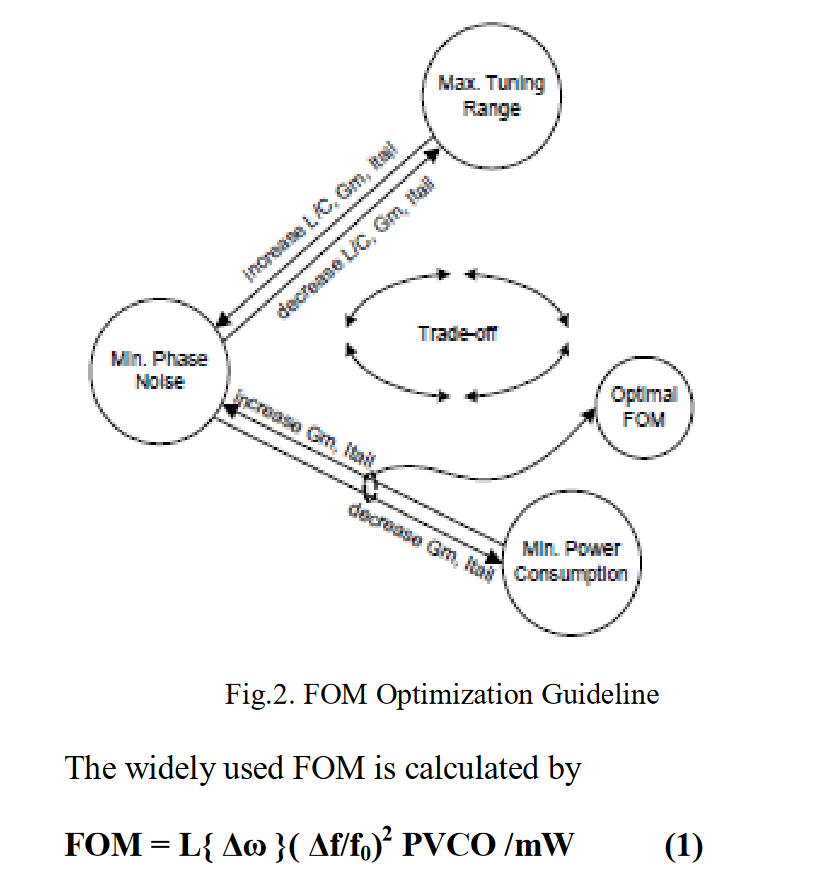
\includegraphics[width=0.5\linewidth]{Figures/vco-tradeoff.png}
	\caption{VCO FoM Optimization and Definition}
	\label{fig:vco-tradeoff}
\end{figure}

% Only VCO design inquiries
% \begin{itemize}
% 	\item (OBSOLETE) hard-clipped VCO not oscillating at the frequency that is supposed to, drops down to around 1 GHz (example)
% 	\item (OBSOLETE) soft-clipped VCO has more frequency modes - CM and DM resonance
% 	\item Reliability of design, breakdown voltages. TDDB is Time Dependent Dielectric Breakdown. 
% 	\item making a differential varactor instead of the single-ended one
% 	\item What is the name of metal stack process to be used in EM simulations?
% \end{itemize}

% \subsection*{Planning to do at some point}

% \begin{itemize}
% 	\item design a 400 to 500 \unit{pH} inductor (search for a paper that has decent Q factor around 4-8 GHz range) % watch out for electromigration, find the paper that I looked at long time ago
% 	\item design a PTAT bandgap voltage reference to switch the gate from cascaded NMOS to reference
% 	\item make a test bench for frequency pushing and frequency pulling (look at the old VCO project)
% 	\item (DOWNTHELINE) Peak Detector
% \end{itemize}

% \begin{question}[\itshape How did we address problems from 2020 feasibility study?]
	% - We did not.
% \end{question}

% Technical Requirements

\subsubsection*{VCO test methods}

\href{https://edisciplinas.usp.br/pluginfile.php/8192379/mod_resource/content/0/VCO-Test_Methods_VCO15-15.pdf}{\textbf{Mini Circuits VCO test methods}} explains how to measure and set up tests for:

\begin{itemize}
	\item output power and frequency
	\item tuning sensitivity and linearity
	\item harmonics and spurious level
	\item frequency pushing
	\item frequency pulling
	\item modulation bandwidth
	\item modern method using a powerful VCO/PLL test system HP4352S
	\item phase noise
\end{itemize}

About modern method: HP has recently introduced a powerful VCO/PLL test system, the HP4352S which is pictured in Figure 4(a). It has built-in low noise power supplies and is available for VCO testing. It measures VCO characteristics such as frequency, tuning linearity, output power, and harmonics as a function of tuning voltage. It can also be used to measure pushing, output power vs. Vcc, phase noise at a given offset vs. VtUne or Vcc, etc. The instrument is user friendly and does not need calibration. A set up using this instrument is illustrated in Figure 4(b). FIGURES NOT SHOWN\\


\newpage

\subsection{Technical requirements}

\begin{table}[ht]
	\centering
	\begin{tabular}{|c|l|c|c|c|c|c|}
		\hline
		& LO Requirements & Note & min & typ & max & Units \\
		\hline
		& \multicolumn{6}{|c|}{\textbf{VCO Requirements}} \\
		\hline
		1 & Full LO range &  & 4000  &  & 8000 & MHz \\ 
		\hline
		1a & Number of cores &  &   & 2 & 4 & / \\ 
		\hline
		2 & Phase Noise at 1 MHz &  &  &  & <-135 & dBc/Hz \\ 
		\hline
		3 & differential Vtune &  & 0.1 &  & Vdd-x & V  \\ % differential
		\hline
		4 & Tuning Sensitivity $K_{VCO}$ &  & ?<30 &  & ?< 50 & MHz/V  \\ 
		\hline
		5 & Pushing & TBD &  &  & 2 & MHz/V  \\ 
		\hline
		6 & Output Voltage p-p & TBD & 0.8 &  & & $V_{p-p}$  \\ 
		\hline
		7 & Load Impedance &  &  &  & 100 & fF  \\ 
		\hline
		& \multicolumn{6}{|c|}{\textbf{VCO and output Buffer}} \\
		\hline
		8 & Output Voltage & TBD & ?0.8  &  &  & $V_{p-p}$ \\ 
		\hline
		9 & Load Impedance & TBD &  &  & ?1000 & fF  \\ 
		\hline
		10 & Harmonic suppression ($2_{nd}$, typ) &  & -15 &  &  & dBc  \\ 
		\hline
		11 & Pulling (14 dB Return Loss, Any Phase) & TBD &  &  & 2 & MHz  \\ 
		\hline
		& \multicolumn{6}{|c|}{\textbf{General Specifications}} \\
		\hline
		12 & Operating Temperature Range &  & -40 &  & 105 & °C  \\ 
		\hline
		13 & Supply Voltage ($\pm 5\%$) &  & 2.375 & 2.5 & 2.625 & V  \\ 
		\hline
		14 & Supply Current &  &  &  & ?20 & mA  \\ 
		\hline
		15 & Shutdown Current &  &  &  & ?10 & $\mu$A  \\ 
		\hline
		16 & Time to Switch Between Cores  &  &  & ?3 & ?5 & ms  \\ 
		\hline
	\end{tabular}
	\label{table-spec-ultra-low-noise}
	\caption{Specification Requirements} 

\end{table}

% FTR - fine tuning range in percentage

\subsection{VCO Design}

\begin{itemize}

	\item What is minimum phase noise that can be obtained with perfect supply, typ process, 25 degC, measured at the VCO output with ideal termination and no buffer
	\item What is the maximum  tuning sensitivity that can be used to obtain the above
	\item What additional techniques need to be explored to improve the above
	\item Perform noise sensitivity analysis like ISF
	\item Discuss CML buffer concept and LDO topologies % LDO will be external
	
\end{itemize}

Previous open points on VCO:

\begin{itemize}
	\item the effects of BSE on phase noise (i.e. is it really needed)
	\item there is no point in using higher resistances than 20 - 30 k$\Omega$ in capacitor bank unit
	\item test voltage and current for HV\_MOSFETs, to test breakdown of mosfets, use software called \textbf{Real Expert} 
	% has to do with SOA (Safe operating area) not being a rectangle
	% find SOA graph in Grujic slides
	\item estimate for drop in phase noise with supply noise and layout and its generous is -120 dBc/Hz % estimate donw by Samuel
	\item to further help needs to review design
\end{itemize}



% I searched relevant papers for VCO 130 nm BiCMOS or similar technologies and frequency range, and haven't found performance even close to 130 dBc @ 1 Mhz offset. 

% \begin{question}[\itshape Based on what was this technology picked for this specification?]
% 	Based on previous feasibility study.
% \end{question}

% \begin{question}[\itshape What is the input reference frequency of PLL? Are there any dividers in PLL?]
% 	Input reference frequency is from 1 GHz to 8 GHz. There are for sure even if the VCO is (4-8 GHz), 2 and 3 dividers are needed.
% \end{question}

% \begin{question}[\itshape Is the input from loop filter single ended or differential?]
% 	It's differential. It also makes more sense for phase noise performance ?!
% \end{question}

% \begin{question}[\itshape How will the PLL lock be detected?]
% 	-
% \end{question}

% Deadbit control is a novel technique to lower settling time.

% Moved to table with technical specifications 

% \begin{question}[\itshape Any estimate for specified VCO output swing?]
% 	-
% \end{question}

% I just realize that BSE should be called LBE (localized backside etch).

\begin{itemize}

	\item [A] another question to the customer regarding the overall system. 8 is a great number for a divider, but maybe a bad choice for a multiplier? I don't know how it is currently implemented, but thinking of diodes/BJT with exponential characteristics we get odd harmonics, using MOS we may get even ones, at least a good 2nd. But 8=2*2*2 and 9 is just 3*3 .. one stage less, and in differential design only 9 seems feasible. In that case I tend to say that a non-sinusoidal output would even help to reduce gain in the multipliers (which also adds noise on top of the multiplication itself). Assuming that the mixer needs amplification, each *2 stage should add more than 6dB PN, leading to about 20dB or more degradation. If they want to have options on that multiplication factor, we could more easily do that in the PLL with dividers (which reduce PN). Ideally we reduce the VCO range to just more than an octave in the highest band of interest and divide the rest?
 
\end{itemize}

% Make two chips (probably for different options for VCO)
% \\
% Test bench to lock PLL, PFD loop filter and VCO.
% \\

% pdk does not support detail inductor modeling.
% \\

% harmonic filter is not included
% \\

% loop bandwidth reallistic that can be achieved internally is from 3 MHz to 100 MHz.
% \\

% up to you if it is 2nd or third order.
% \\






\subsection{Using different models for HBT}

BSIM4 and psp* (not pss), sometimes psp* gives better performance
% TOSEARCH for how "psp" models are really called?

BSIM4, as the extension of BSIM3 model, addresses the MOSFET physical effects into sub-100nm regime. The continuous scaling of minimum feature size brought challenges to compact modeling in two ways: One is that to push the barriers in making transistors with shorter gate length, advanced process technologies are used such as non-uniform substrate doping. The second is its opportunities to RF applications.


% \subsection{Regarding VCO design option 2 results}

% I have simulated pnoise for designs and testbenches Gunther sent me and I don't get the same results.

% I believe simulation using setting multiplenoise that gives phase noise perfrmance that is now being presented is not correct.
% As for multiple different nets it gives very different values, which makes little sense with the topology.
% And when I use only one output noise for pnoise simulation I get much worse results (15-20 dBs), but they are consistent.

% Sorry to bring other people into this, I thought this is important and I wanted to remove myself from these results presented since I also spent some time simulating this design this past week.

% Also for the design Gunther sent me today. The results I got with his testbench:

% These are not normalized results so they are 5-6 dBs lower, but still far from what was expected.

% rfOutputNoise("dBc/Hz" ?result "pnoise")


% \subsection{Tasks regarding the VCO option 2 and 1}

% option 2

% Review VCO option 2 BJT and CMOS options \\
% Review PFD latest results and CP status \\
% Review approach going forward and schedule proposals \\

% Guenter/Aleksandar/Anthime, can we have for each of the blocks (VCO1a, VCO1b, PFD/CP) a status page showing: \\
% performance summary (if different than the VCO comparison table) \\
% any special needs (supply, BSE etc) \\
% projected area \\
% risks so far

\subsection{Problem with discontinuity of RF model}

When simulating design with nmosHVRF models this error appears:

\begin{verbatim}
WARNING (SPECTRE-16780): LTE tolerance was temporarily relaxed to step over a 
		discontinuity in the signal: i_VCO.i_VCO_core.N3:int_INT3. Check the design 
		or use '+diagnose' to get more information.
        Further occurrences of this warning will be suppressed
\end{verbatim}

I changed the model parameter:
\begin{verbatim}
	+ swnqs         =  0.0 * rfmode * 5.0
	In section of sg13g2_moshv_psp_parm.scs/ 
	sg13g2_hv_nmos / model sg13g2_hv_nmos_psp pspnqs103.		
\end{verbatim}

\subsection{30 GHz VCO design}
by Stefan Jović
% with divider by 4 

Performance summary:
\begin{table}[ht]
	\centering
	\begin{tabular}{|c|c|}
		\hline
		Parameter & Typical value \\
		\hline
		Corner & Typical \\
		\hline
		Temperature & 50 °C \\
		\hline
		Amplitude & ~ 550 mVpp \\
		\hline
		Centre Frequency & ~ 30.25 GHz \\
		\hline
		Tuning Range & ~ 0.72 GHz \\
		\hline
		$K_{VCO}$ & ~ 1.45 GHz/V \\
		\hline
		Tuning range voltage & 0.2 V - 0.7 V \\
		\hline
	\end{tabular}
	\label{30GHz-VCO-design}
	\caption{Specification Requirements} 
\end{table}

Some key conclusions in terms of phase noise:

Noise at output of VCO is same as at the output of buffer. Main contributors for VCO output noise is output buffer by performing modulation of VCO tank circuit. Second main contributor is noise in references used to generate VCO current bias and noise in power supply.

Note that current tail bias mirror is using PTAT current.

\begin{question}[\itshape Why is PTAT used?]
	VCO output swing or VCO output freq or sth else?
\end{question}


\subsection{VCO sub blocks and relevant blocks}

List of sub blocks:

\begin{itemize}
	\item VCO core (\# is 8 for BiCMOS)
	\item Differential tuning circuit - varactor (bank)
	\item Capacitor bank
	\item Current or Voltage Bias
	\item Bandgap Reference
	\item Output Buffer
\end{itemize}


% asked for a showcase of source degeneration - response, that it does not actually help

%----------------------------------------------------------------------------------------
%	DESIGN OF VCO TANK
%----------------------------------------------------------------------------------------

\subsection{Design of VCO Tank}

% TOLOOK Design of transformer based tank - Noise Circulating VCO 

\subsubsection{Differential Varactor}
%
2 papers \\

Option 1 is referencing \href{https://ieeexplore.ieee.org/document/1494046?arnumber=1494046}{\textbf{paper}} A 44 \unit{GHz} Differentially Tuned VCO with 4GHz Tuning Range in 0.12 \unit{um} SOI CMOS


\begin{figure}[ht!]
	\centering
	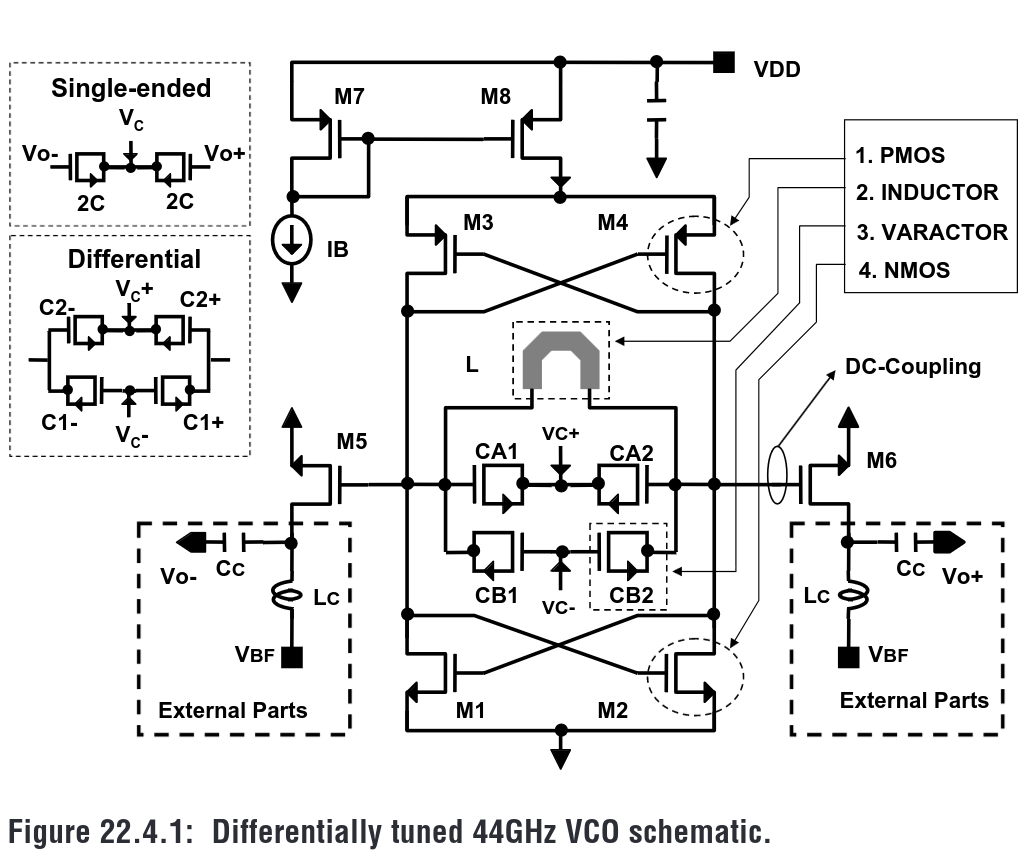
\includegraphics[width=0.5\linewidth]{Figures/diff-var1.png}
	% \caption{Difference between class C and class B}
	\label{fig:diff-var1}
\end{figure}

Option 2 is referencing \href{https://ieeexplore.ieee.org/document/9056968}{\textbf{paper}} A 23-mW 60-GHz Differential Sub-Sampling PLL with an NMOS-Only Differential-Inductively-Tuned VCO
\begin{figure}[ht!]
	\centering
	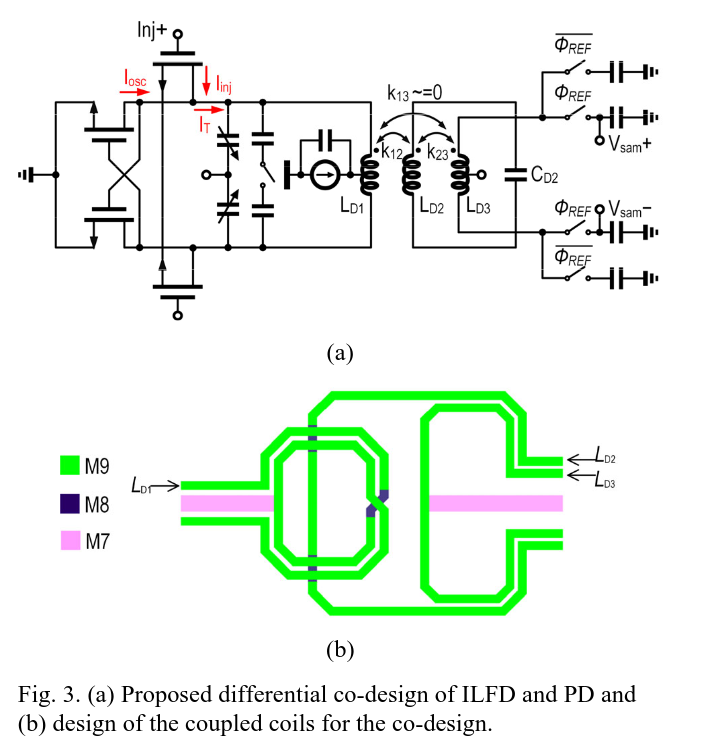
\includegraphics[width=0.5\linewidth]{Figures/diff-var2.png}
	% \caption{Difference between class C and class B}
	\label{fig:diff-var2}
\end{figure}

low Q part of Varactor tuning range: % don't know what i wanted to write

Testbench for comparing differential and single-ended tuning:

\begin{figure}[ht!]
	\centering
	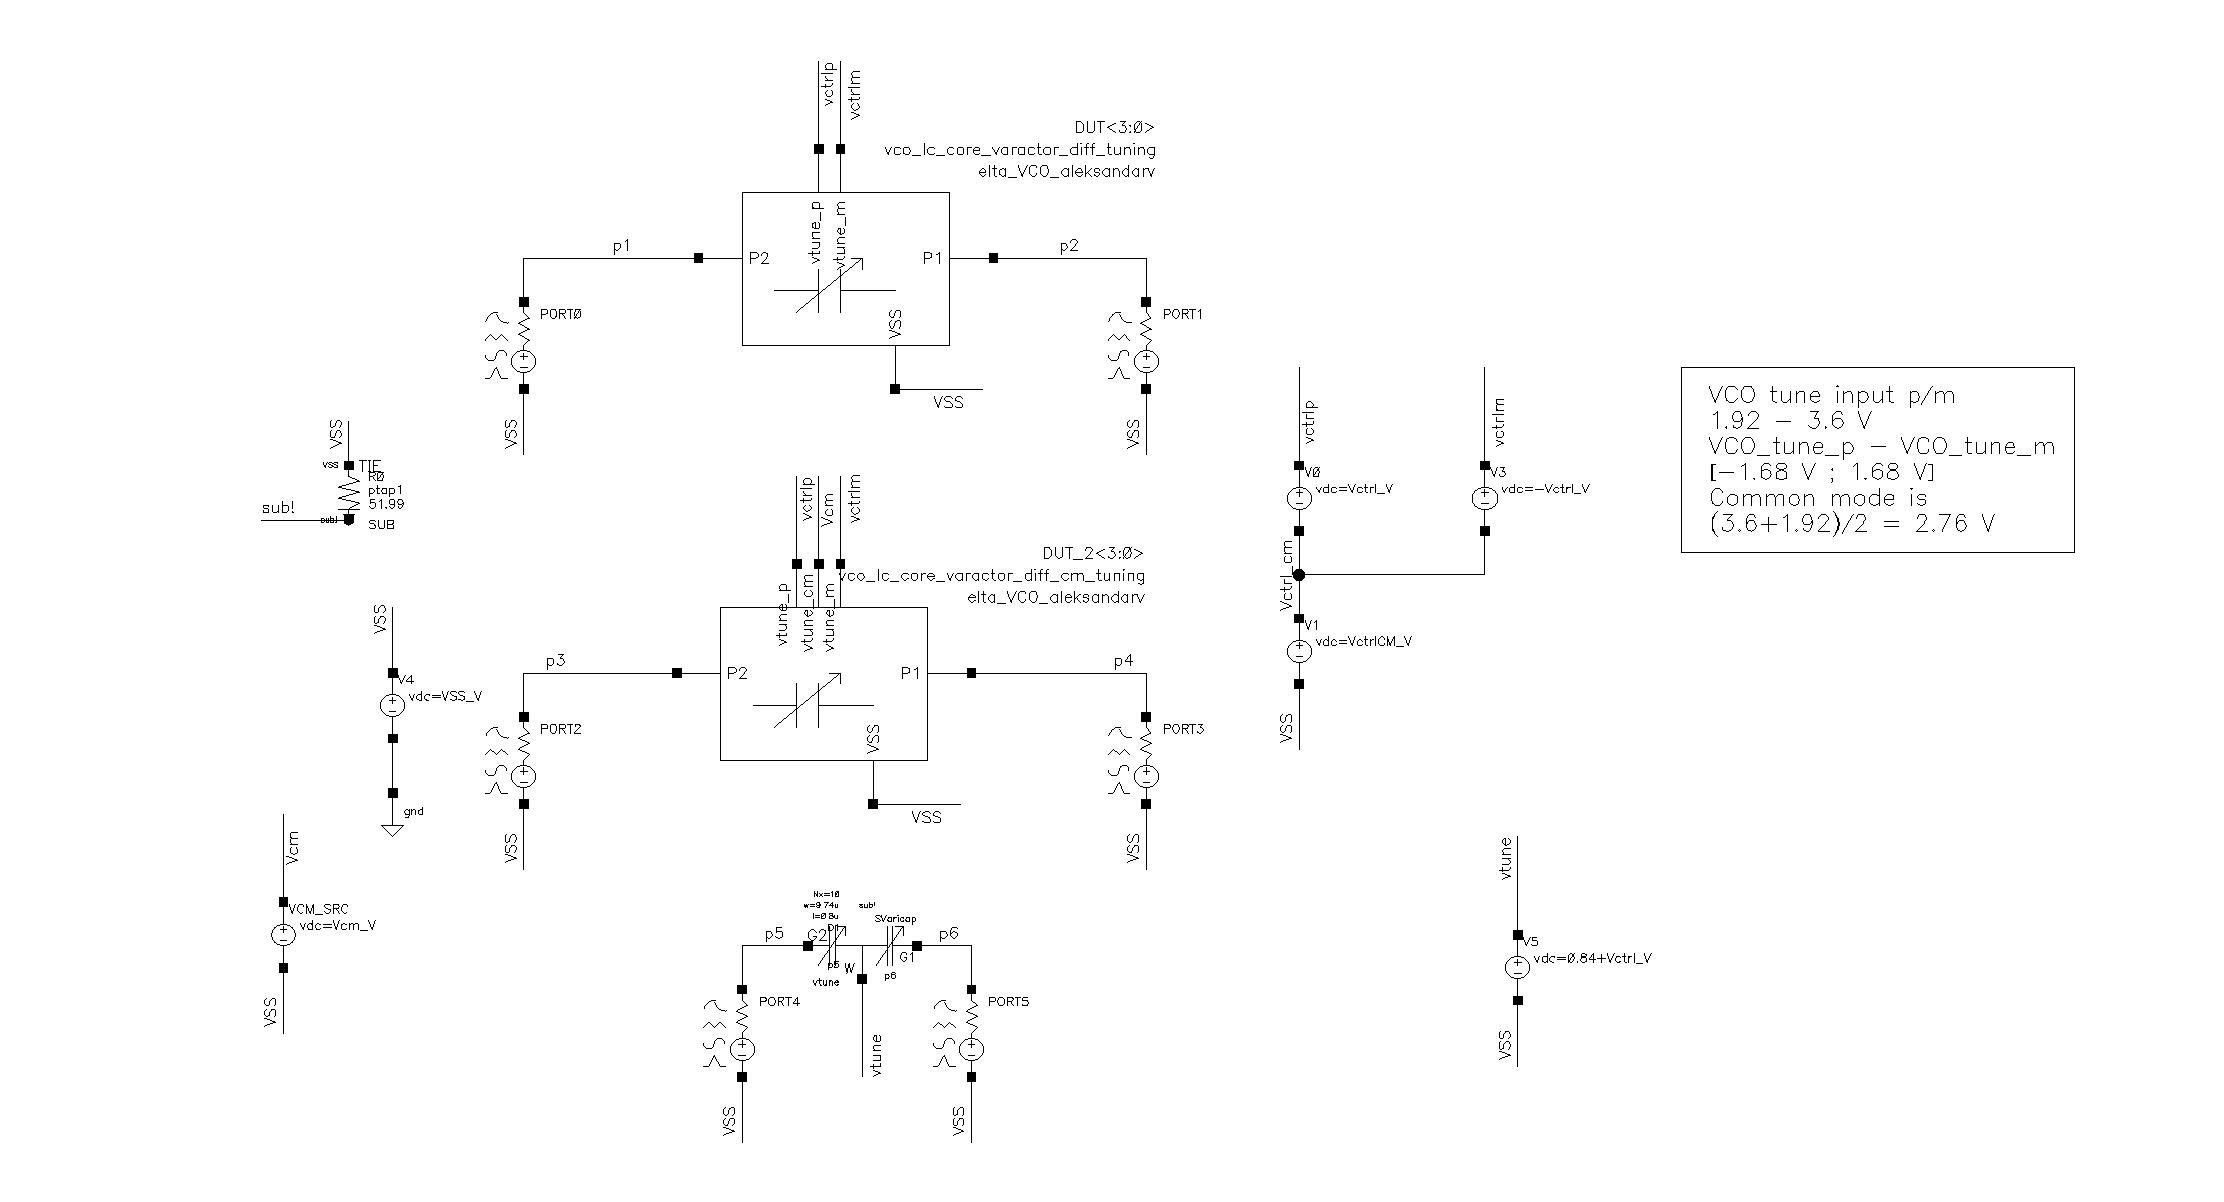
\includegraphics[width=\linewidth]{Figures/cvar-testbench.jpg}
	\caption{Testbench for capacitive varactors}
	\label{fig:cvar-testbench}
\end{figure}

Results of comparative analysis.

\begin{figure}[ht!]
	\centering
	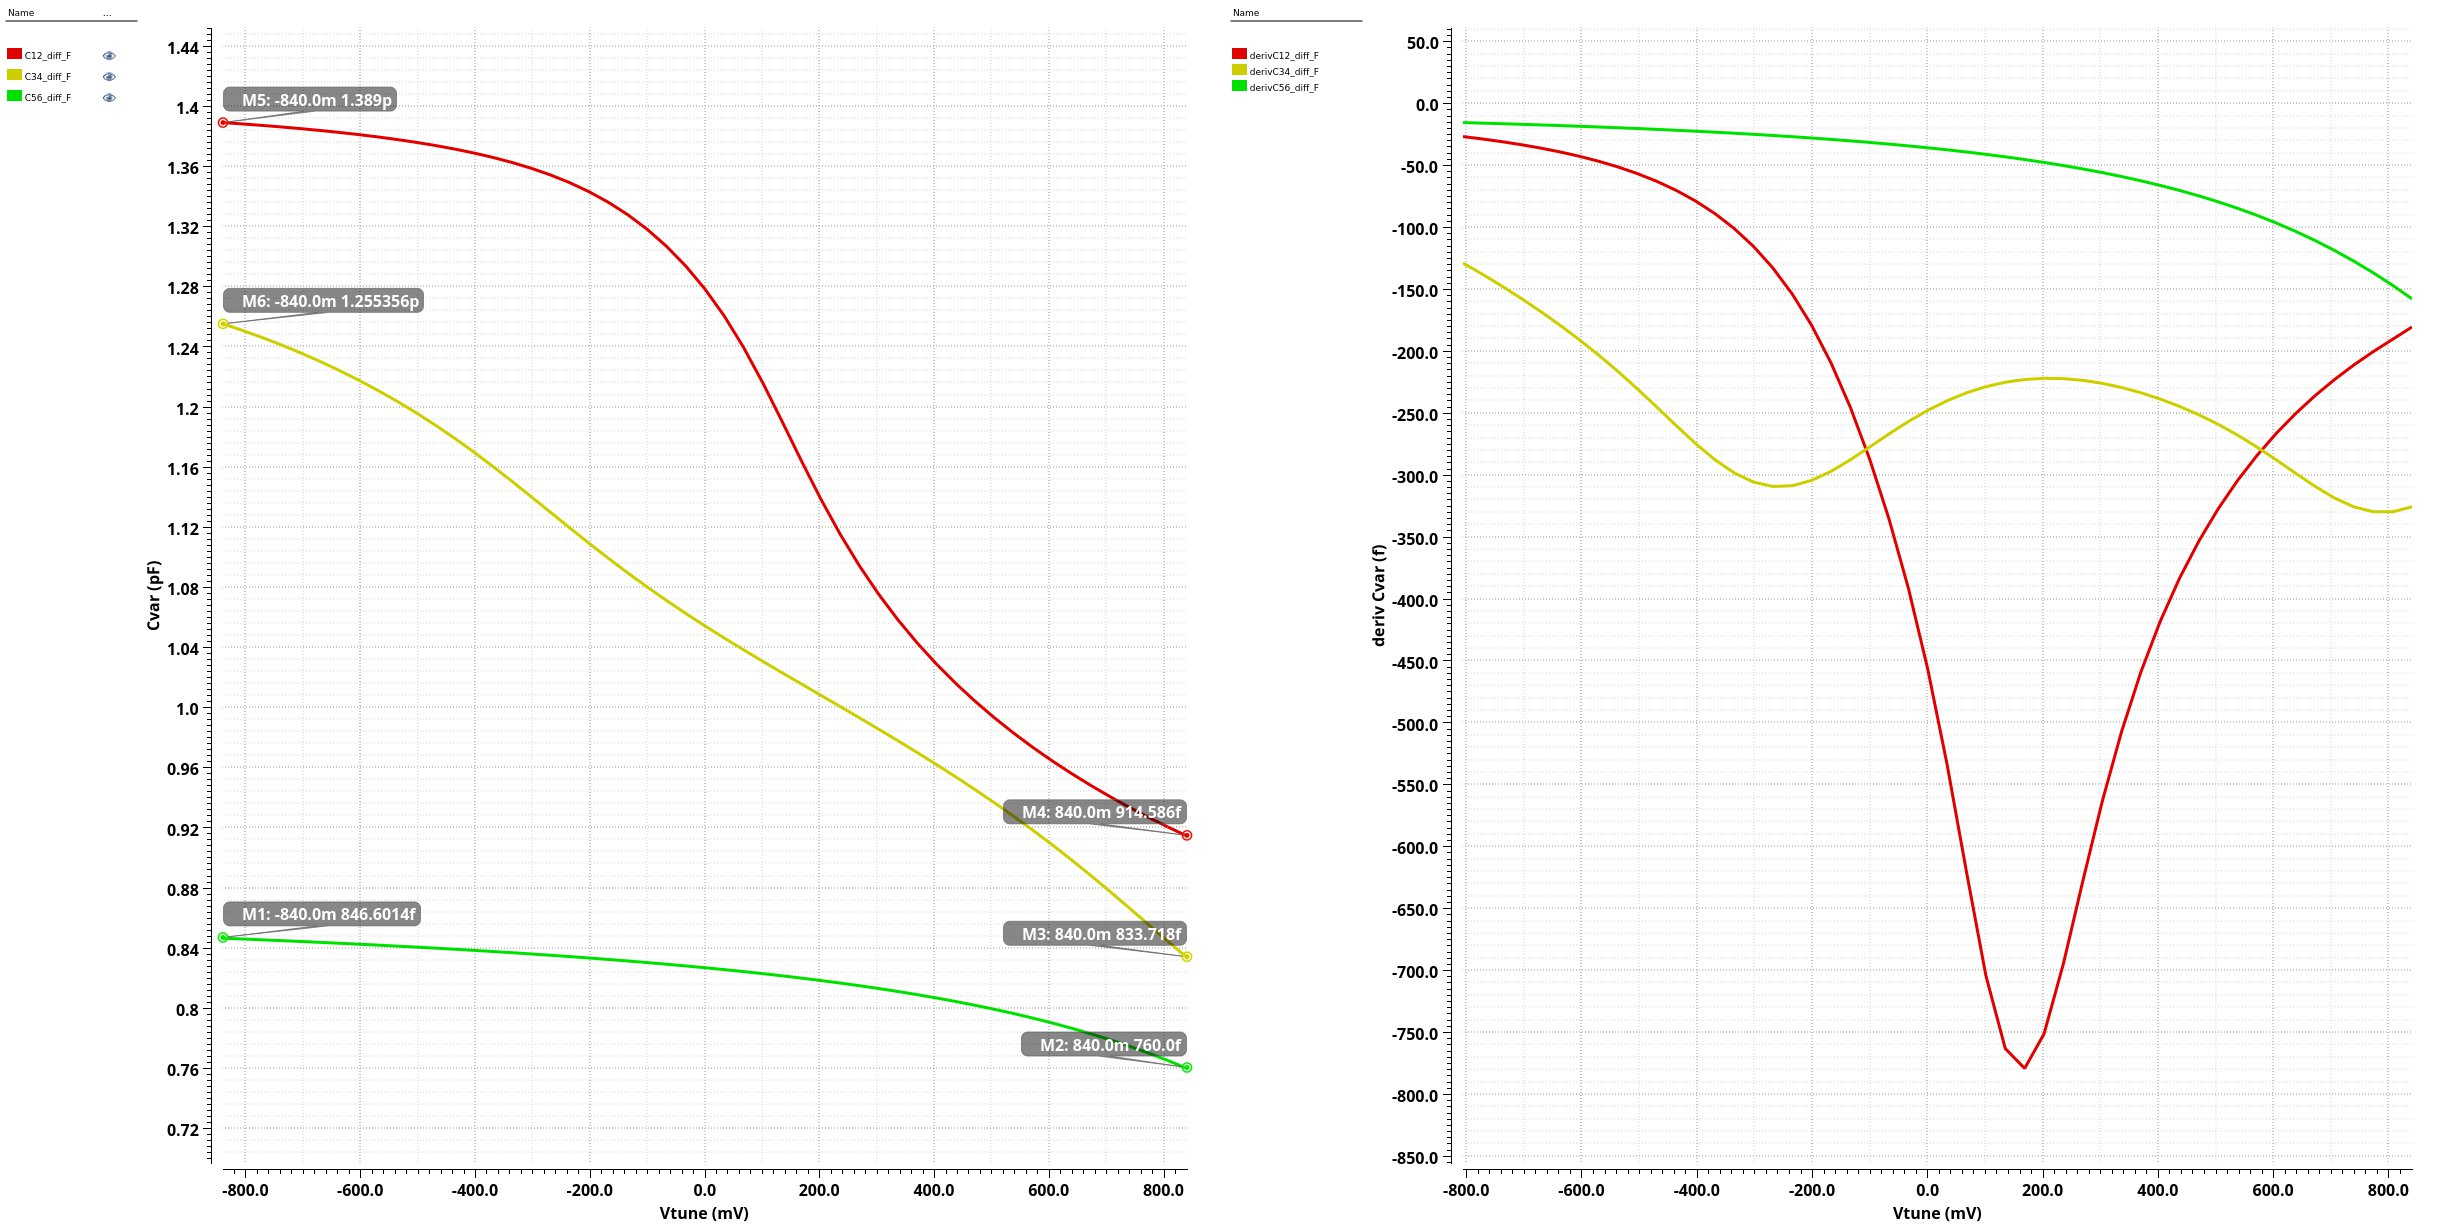
\includegraphics[width=\linewidth]{Figures/cvar-sweep-over-vtune-comparison.jpg}
	\caption{Simulation Results Cvar and deriv(Cvar) over Vtune}
	\label{fig:cvar-sweep-over-vtune-comparison}
\end{figure}

Regarding linearity of differential tuning (I assume you are talking about this), I could not figure this out, and opted for single-ended tuning. The problem is that differential tuning has less capacitance change and inherently loads tank with more capacitance, resulting in lower VCO frequency which results in lower phase noise when normalized to 7 GHz, and also lower tuning range.


Red and yellow are differential "varactors" and green C56 is single-ended. On the left is sweep of tunging voltage to see change in capacitance, on the right derivative of this - indicates KVCO and "linearity".
Yellow is more "linear" than red and  it uses "common mode voltage" Vtunecm = VDD, while red one is the simple one.

This is the schematic for the yellow $C_{34}$ one $vtune_{cm}$ is connected to supply.

Red plot represents this differential "varactor" without cm voltage C12.




% \begin{info}
	
% \end{info}

Q factor is worse for differential tuning vs single-edned tuning.

\subsubsection{Design of Capacitor Bank and CB Unit} % or Banks  

2 Single-ended banks vs Differential capacitor banks

\subsubsection{Design of Inductor}

Electro-magnetic simulator is needed. Technology Parameters if calculations are to be done. Look up the metal stack and info % where to find this

\begin{table}[ht]
	\centering
	\begin{tabular}{|c|c|c|}
		\hline
		Parameter & Value & Unit \\
		\hline
		\hline
		Substrate resistivity & X & $\Omega$-\unit{cm}\\
		\hline
		Substrate thickness & ? & $um$ \\
		\hline
		Silicon dielectric constant & ? & no unit \\
		\hline
		Oxide thickness (M3-Sub) & ? & $um$ \\
		\hline
		Oxide thickness (M3-M2) & ? & $um$ \\
		\hline
		$SiO_2$ dielectric constant & ? & no unit \\
		\hline
		Metal resistivity & ? & $\Omega$-\unit{um} \\
		\hline
		Top Metal (M?) thickness & ? & $um$ \\
		\hline
		Other metal thickness& ? & $um$ \\
		\hline
	\end{tabular}
	\label{tech-param}
	\caption{Technology Parameters} 

\end{table}

Inductor can be also switchable, if we need to improve the crude tuning range.

